
\subsection{L'Application Checkers}

l'application Checkers (principe), décompilation, un bytecode obscure
dex2jar, jd-gui, correction des erreurs, éclaircissement du code, une archi mvc.
Fonctionnement de l'appli en interne
\subsubsection{Principe}

\subsubsection{Décompilation et analyse du code}

\subsubsection{Architecture}
Dans un point de vue général, le développeur du jeu Checkers a adopté une architecture MVC. Ce qui nous a beaucoup aidé à determiner les différentes 
classes. 
\begin{figure}[hp]
	      \begin{center}
		\fbox{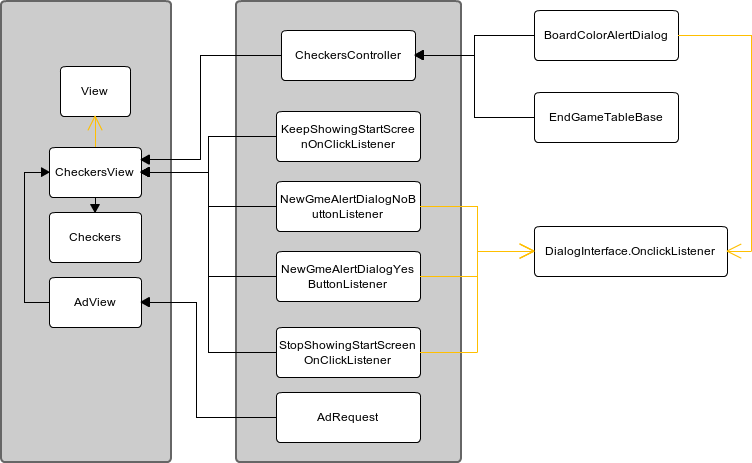
\includegraphics[scale=0.7]{archi}}
	      \end{center}
	\legend{architecture}
\end{figure}
